% === SET DOCUMENT METADATA ===
\def\docTitle{Technical Design Document (TDD)}
\def\docVersion{3.1}
\def\docDate{July 19, 2026}

% === INCLUDE REUSABLE COMPONENTS ===
% === PACKAGES ===
\documentclass[12pt,a4paper]{report}
\usepackage[utf8]{inputenc}
\usepackage[T1]{fontenc}
\usepackage{geometry}
\geometry{left=2.5cm,right=2.5cm,top=2.5cm,bottom=2.5cm,headheight=24.65pt,footskip=1.5cm}
\usepackage{graphicx}
\usepackage{xcolor}
\usepackage{fancyhdr}
\usepackage{titlesec}
\usepackage{hyperref}
\usepackage{enumitem}
\usepackage{tabularx}
\usepackage{longtable}
\usepackage{array}
\usepackage{listings}
\usepackage{float}   % For [H] placement

% === BRANDING COLOR ===
\definecolor{mooveblue}{RGB}{0, 87, 184}
\definecolor{codegray}{RGB}{240, 240, 240}

% === HEADER / FOOTER SETUP ===
\pagestyle{fancy}
\fancyhf{}
\renewcommand{\headrulewidth}{1pt}
\renewcommand{\headrule}{\hbox to\headwidth{\color{mooveblue}\leaders\hrule height \headrulewidth\hfill}}

% Footer: Page number in center, left/right text for context
\fancyfoot[C]{\thepage}
\fancyfoot[L]{\textit{Confidential - Internal Use Only}}
\fancyfoot[R]{\textit{Contains Apache 2.0 Licensed Code}}

% === SECTION STYLING ===
\titleformat{\section}{\normalfont\Large\bfseries\color{mooveblue}}{\thesection}{1em}{}
\titleformat{\subsection}{\normalfont\large\bfseries\color{mooveblue}}{\thesubsection}{1em}{}
\titleformat{\subsubsection}{\normalfont\normalsize\bfseries\color{mooveblue}}{\thesubsubsection}{1em}{}
\titleformat{\paragraph}[runin]{\normalfont\normalsize\bfseries\color{mooveblue}}{\theparagraph}{1em}{}

% === CODE LISTING STYLE ===
\lstset{
    backgroundcolor=\color{codegray},
    basicstyle=\footnotesize\ttfamily,
    breaklines=true,
    frame=single
}

% === FOOTER OVERRIDE ===
\fancyhead[L]{\textcolor{mooveblue}{\textbf{Moove Education Platform}}}
\fancyhead[R]{\textbf{TDD v3.0}}

% === BEGIN DOCUMENT ===
\begin{document}

% === COVER PAGE ===
\begin{titlepage}
    \centering
    \vspace*{1cm}
    
\includegraphics[width=5cm]{../logo.png}\\[1cm]
    {\Huge \textbf{Moove Education Platform}}\\[0.5cm]
    {\Large \docTitle}\\[0.5cm]
    {\large Version \docVersion}\\[0.2cm]
    {\large \docDate}\\[1.5cm]
    
    \textbf{Prepared By:}\\
    Moove\\
    \vfill
    \textit{This product includes software from the Open edX project, licensed under Apache 2.0.}\\
    \today
\end{titlepage}

\tableofcontents
\newpage

\section{API Specification}
The platform exposes REST APIs (EdX API v1, OAuth2) with security controls aligned to INSA requirements. Key endpoints are documented below.

\subsection{Authentication and Authorization}
\begin{itemize}
    \item All API endpoints require authentication via OAuth2 or JWT (CMCSRS 6.17).
    \item Basic Authentication is disabled in production.
    \item Access tokens have a limited lifetime and are refreshed using refresh tokens.
    \item Role‑based access control (RBAC) is enforced for all endpoints.
\end{itemize}

\subsection{Rate Limiting and Throttling}
\begin{itemize}
    \item Rate limiting is applied to prevent brute‑force attacks (fail2ban and Django throttle).
    \item Login endpoints are limited to 5 attempts per minute per IP.
\end{itemize}

\subsection{Input Validation and Output Encoding}
\begin{itemize}
    \item All user input is validated and sanitised to prevent SQL injection, XSS, and command injection.
    \item Output is properly encoded to prevent XSS.
\end{itemize}

\subsection{Key Endpoints}
\begin{itemize}
    \item \texttt{/api/user/v1/} – User management (requires OAuth2).
    \item \texttt{/api/courses/v1/} – Course listing and enrollment (requires authentication).
    \item \texttt{/api/gradebook/v1/} – Grade retrieval (requires appropriate role).
    \item \texttt{/api/discussion/v1/} – Forum threads and posts (requires authentication).
    \item \texttt{/api/analytics/v1/} – Usage reports (instructor only).
    \item \texttt{/api/certificates/v1/} – Certificate generation (requires verified enrollment).
\end{itemize}

For detailed API schemas, see the Swagger documentation (swagger-docs.json).

\section{Database Schema}
The database design incorporates security and privacy by design.

\subsection{Entity-Relationship Diagram}
\begin{figure}[H]
\centering
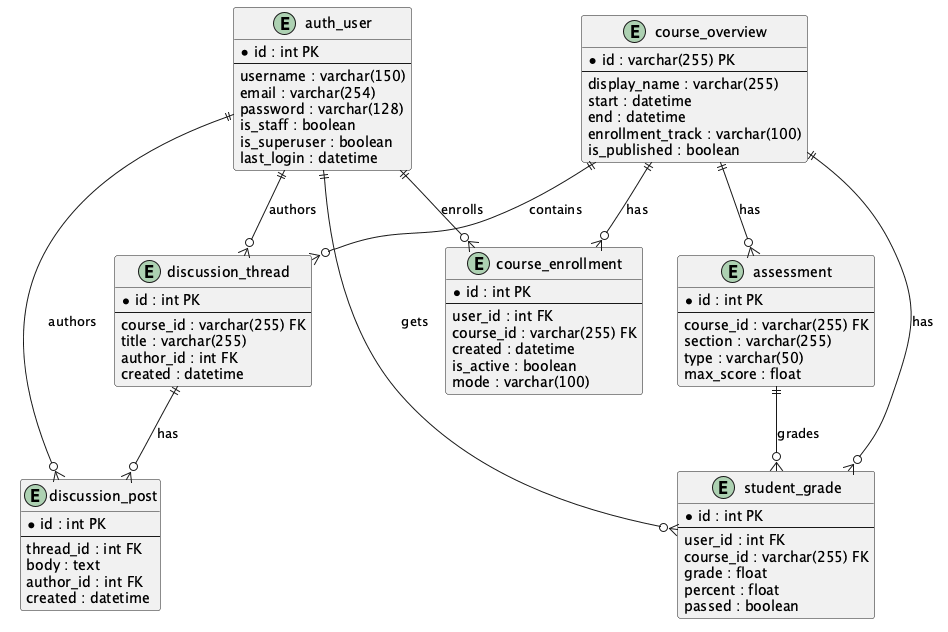
\includegraphics[width=\textwidth,height=0.7\textheight,keepaspectratio]{diagrams/er.png}
\caption{ER Diagram showing primary tables.}
\end{figure}

\subsection{Key Tables with Security Considerations}
\begin{itemize}
    \item \texttt{auth\_user}: id, username, email, password\_hash (bcrypt), is\_staff, is\_superuser.
    \item \texttt{course\_overview}: id, display\_name, start, end, enrollment\_track.
    \item \texttt{course\_enrollment}: id, user\_id, course\_id, created, is\_active.
    \item \texttt{student\_grade}: id, user\_id, course\_id, grade, percent.
    \item \texttt{discussion\_thread}: id, course\_id, title, author\_id, created.
    \item \texttt{discussion\_post}: id, thread\_id, body (sanitised), author\_id, created.
    \item \texttt{certificate\_generated}: id, user\_id, course\_id, created, download\_url (signed URL).
    \item \texttt{team}: id, course\_id, name, description, topic.
    \item \texttt{team\_membership}: id, team\_id, user\_id, role.
    \item \texttt{bookmark}: id, user\_id, course\_id, content\_id, created.
\end{itemize}

\subsection{Data Protection Measures}
\begin{itemize}
    \item Sensitive fields (email, password hash, personal data) are encrypted at rest using AES‑256.
    \item Database backups are encrypted and stored separately.
    \item Audit logs are maintained for all critical database operations (user creation, role changes, grade updates).
\end{itemize}

\section{Design Traceability}
The following table maps requirements to API endpoints and database tables, with security annotations.

\begin{longtable}{|p{3cm}|p{4cm}|p{3cm}|}
\hline
\textbf{Requirement ID} & \textbf{API Endpoint(s)} & \textbf{Table(s)} \\
\hline
\endfirsthead
\hline
\textbf{Requirement ID} & \textbf{API Endpoint(s)} & \textbf{Table(s)} \\
\hline
\endhead
\hline
\multicolumn{3}{|r|}{Continued} \\
\hline
\endfoot
\hline
\endlastfoot
UFR-OE-001-01 & POST /api/courses/v1/courses & course\_overview \\
UFR-OE-001-03 & POST /api/enrollment/v1/enrollment & course\_enrollment \\
UFR-OE-003-01 & GET /api/discussion/v1/threads & discussion\_thread \\
UFR-OE-003-02 & POST /api/email/v1/bulk & (Celery) \\
UFR-OE-004-01 & PUT /api/courses/v1/courses/\{course\_id\}/content & course\_structure \\
UFR-OE-005-03 & POST /api/ora/v1/assessments & ora\_assessment \\
UFR-OE-006-03 & GET /api/gradebook/v1/grades & student\_grade \\
UFR-OE-103-01 & POST /api/enrollment/v1/enrollment & course\_enrollment \\
UFR-OE-107-01 & GET /api/certificates/v1/status & certificate\_generated \\
UFR-OE-109-01 & POST /api/discussion/v1/posts & discussion\_post \\
UFR-OE-113-01 & POST /api/bookmarks/v1/ & bookmark \\
SEC-NFR-001..007 & All endpoints & All tables (with security controls) \\
\hline
\end{longtable}

\section{Activity Diagrams}
\subsection{Activity: Course Publishing}
\begin{figure}[H]
\centering
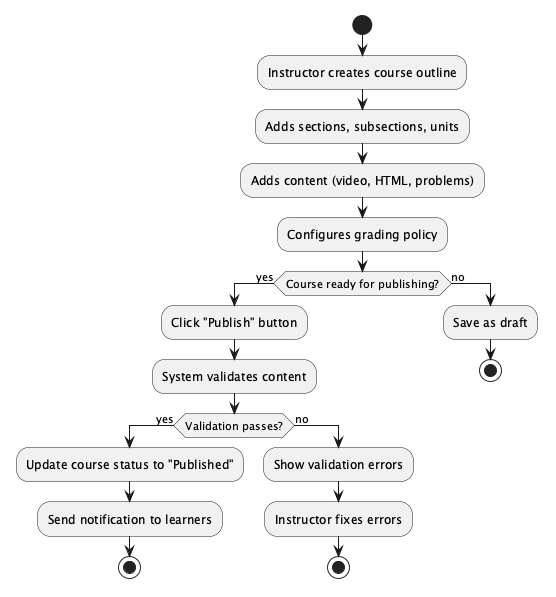
\includegraphics[width=0.7\textwidth,height=0.7\textheight,keepaspectratio]{diagrams/activity_course_publish.png}
\caption{Course publishing workflow.}
\end{figure}

\subsection{Activity: Open Response Assessment}
\begin{figure}[H]
\centering
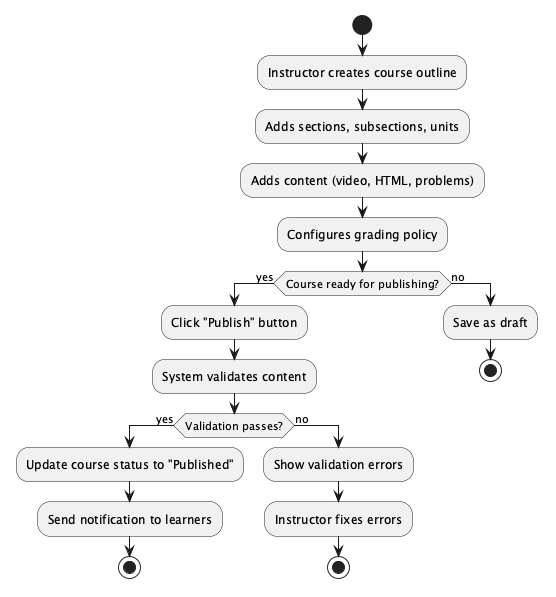
\includegraphics[width=0.7\textwidth,height=0.7\textheight,keepaspectratio]{diagrams/activity_ora.png}
\caption{Open Response Assessment workflow.}
\end{figure}

\section{References}
\begin{itemize}
    \item \textit{Security Architecture \& Threat Model – Moove Education Platform} (Security\_OpenEdX.tex)
    \item CMCSRS v2.0
    \item Swagger API documentation (swagger-docs.json)
\end{itemize}

% === LICENSE ATTRIBUTION ===
\newpage
\section*{Apache License 2.0 Attribution}
This product includes software developed by the \textbf{Open edX Project} (\url{https://open.edx.org/}) licensed under the Apache License, Version 2.0 (\url{http://www.apache.org/licenses/LICENSE-2.0}).

\textit{Moove Education Platform is a derivative work of Open edX. No modifications have been made to the original license terms. A copy of the full license text is available in the root of the source repository and in Appendix A of this document.}

% === OPTIONAL: Include full license in appendix ===
\appendix
\section{Full Apache License 2.0 Text}
\input{../common/license}

\end{document}
\end{document}